% Convolution as a sum of shifted, scaled kick responses.
% Upper panel: the input u(tau) = 2^{-tau} and its slices, each of area u(tau_i) * delta-tau.
% Lower panel: one decaying copy of the kick response phi(t) = e^{-t} per slice, and their sum.
\begin{center}
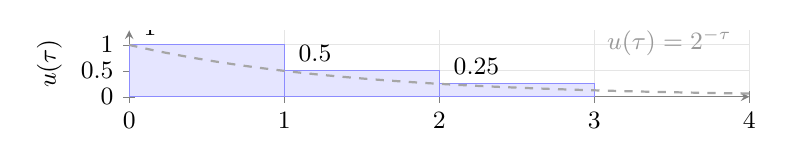
\begin{tikzpicture}
\begin{axis}[
  width=0.78\linewidth, height=0.20\linewidth,
  ylabel={$u(\tau)$},
  axis lines=left,
  axis line style={gray},
  label style={font=\small},
  tick label style={font=\small},
  xmin=0, xmax=4, ymin=0, ymax=1.28,
  xtick={0,1,2,3,4}, ytick={0,0.5,1},
  grid=major, grid style={gray!20},
]
\fill[blue!10] (axis cs:0,0) rectangle (axis cs:1,1);
\fill[blue!10] (axis cs:1,0) rectangle (axis cs:2,0.5);
\fill[blue!10] (axis cs:2,0) rectangle (axis cs:3,0.25);
\draw[blue!45] (axis cs:0,0) rectangle (axis cs:1,1);
\draw[blue!45] (axis cs:1,0) rectangle (axis cs:2,0.5);
\draw[blue!45] (axis cs:2,0) rectangle (axis cs:3,0.25);
\addplot[domain=0:4, samples=100, thick, gray!70, dashed] {2^(-x)};
\node[font=\small, anchor=south west] at (axis cs:0.03,1.0) {$1$};
\node[font=\small, anchor=south west] at (axis cs:1.03,0.5) {$0.5$};
\node[font=\small, anchor=south west] at (axis cs:2.03,0.25) {$0.25$};
\node[font=\small, gray!80, anchor=east] at (axis cs:3.95,1.05) {$u(\tau) = 2^{-\tau}$};
\end{axis}
\end{tikzpicture}

\vspace{0.5em}

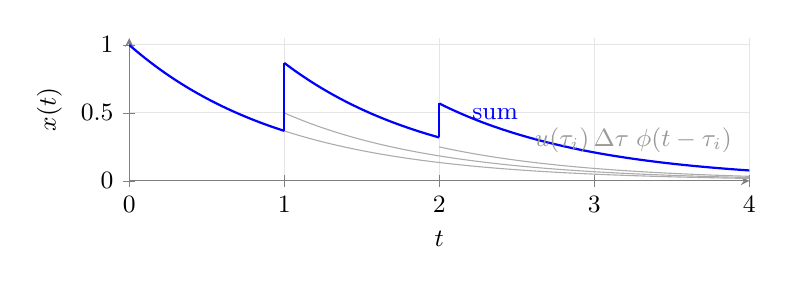
\begin{tikzpicture}
\begin{axis}[
  width=0.78\linewidth, height=0.28\linewidth,
  xlabel={$t$}, ylabel={$x(t)$},
  axis lines=left,
  axis line style={gray},
  label style={font=\small},
  tick label style={font=\small},
  xmin=0, xmax=4, ymin=0, ymax=1.05,
  xtick={0,1,2,3,4}, ytick={0,0.5,1},
  grid=major, grid style={gray!20},
]
\addplot[domain=0:4, samples=200, thin, gray!65] {exp(-x)};
\addplot[domain=1:4, samples=200, thin, gray!65] {0.5*exp(-(x-1))};
\addplot[domain=2:4, samples=200, thin, gray!65] {0.25*exp(-(x-2))};
\addplot[domain=0:1, samples=60, thick, blue] {exp(-x)};
\addplot[domain=1:2, samples=60, thick, blue] {exp(-x) + 0.5*exp(-(x-1))};
\addplot[domain=2:4, samples=120, thick, blue] {exp(-x) + 0.5*exp(-(x-1)) + 0.25*exp(-(x-2))};
\draw[thick, blue] (axis cs:1,0.3679) -- (axis cs:1,0.8679);
\draw[thick, blue] (axis cs:2,0.3193) -- (axis cs:2,0.5693);
\node[font=\small, blue, anchor=north west] at (axis cs:2.15,0.60) {sum};
\node[font=\small, gray!80, anchor=east] at (axis cs:3.95,0.30) {$u(\tau_i)\,\Delta\tau\;\phi(t-\tau_i)$};
\end{axis}
\end{tikzpicture}
\end{center}
